\cia  \vspace{-2cm}
\section{The JANR fit}
The JANR model \cite{bib:Inna1}, \cite{bib:Inna2} incorporates the unitary isobar approach \cite{bib:maid2000}
modified in order to
include the Regge poles. The resonances contribute as Breit-Wigner, while non resonant background is built 
from the
Born terms and the {\it t}-channel $\rho$ and $\omega$ contributions. To calculate the Born terms
the latest calculation of
the nucleon and pion form factors was used. 

The parameters obtained by fitting the cross section data are the magnitudes of the multipoles
corresponding to the resonance from the first and second resonance regions at the resonance positions.
After extracting the multipoles, the JANR program can recalculate the cross section. An example of this process is illustrated
in \F{fig:cro_phi_W1.23_Q23.50_Inn} where both the data (blue triangles) and the JANR cross section (solid black line) are plotted.
The JANR global fit well reproduces the experimental data behaviour. 

\begin{figure}[h]
 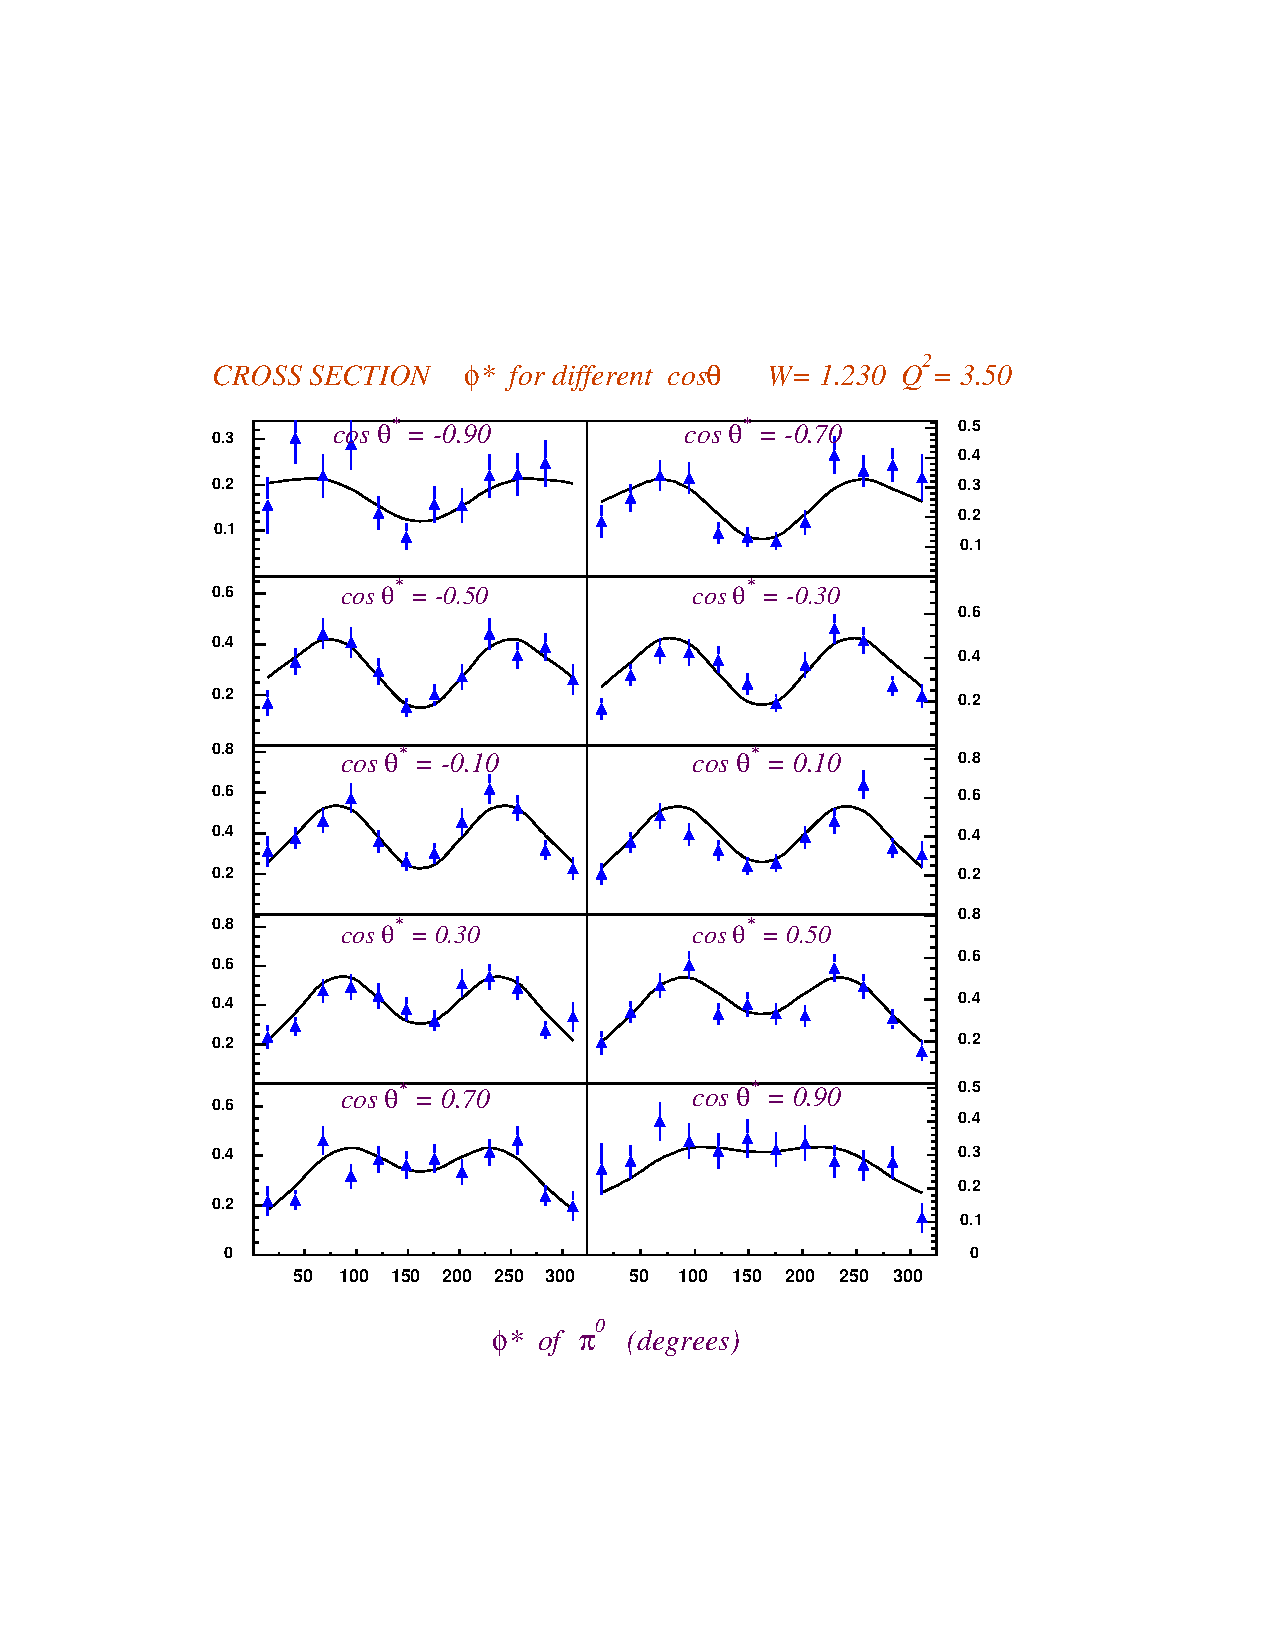
\includegraphics[width = 13cm, bb=-30 140 520 640]{analysis/img/cro_phi_W1.23_Q23.50_Inn}
  \caption[JANR fit of the cross section.]
{ JANR fit of the cross section. The blue triangles represent the experimental data points. The solid black line
 is the JANR calculated cross section after the fit.}
 \label{fig:cro_phi_W1.23_Q23.50_Inn}
\end{figure}

\cia
To further investigate the JANR fit result, the JANR obtained cross section was fitted with Legendre polynomials
as described in \ref{sec:structure}, 
and the structure functions were extracted. An example is shown in \F{fig:lpt_Q23.50_Inn_L1}, 
\F{fig:lt_Q23.50_Inn_L1} and \F{fig:tt_Q23.50_Inn_L1}, where $\sigma_T+\epsilon_L\sigma_L$, $\sigma_{LT}$ and $\sigma_{TT}$ 
are shown respectively.

\begin{figure}[h]
 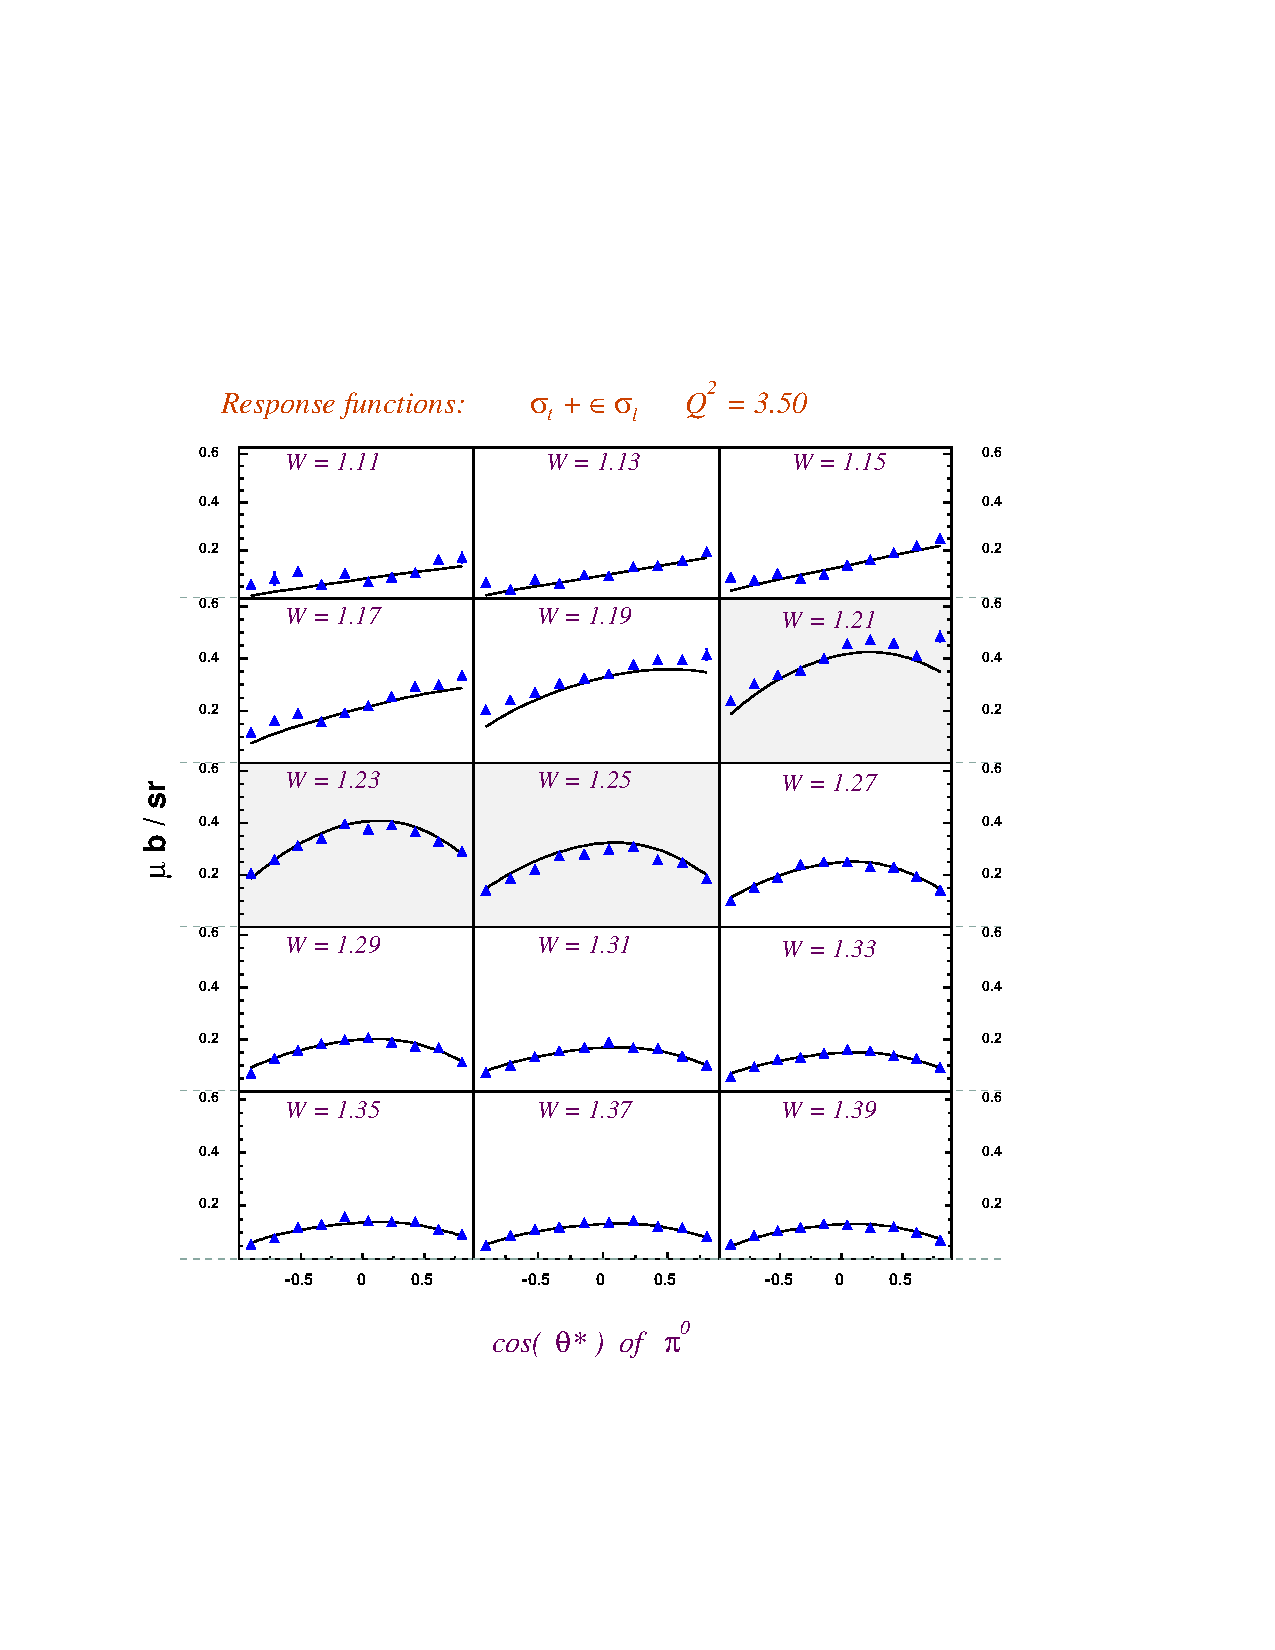
\includegraphics[width = 13cm, bb=-30 140 480 640]{analysis/img/lpt_Q23.50_Inn_L1}
  \caption[JANR fit of the cross section: $\sigma_T+\epsilon_L\sigma_L$]
{ JANR fit and  $\sigma_T+\epsilon_L\sigma_L$. The blue triangles represent the experimental data points. The solid black line
 is the JANR calculated cross section after the JANR fit.}
 \label{fig:lpt_Q23.50_Inn_L1}
\end{figure}

\begin{figure}[h]
 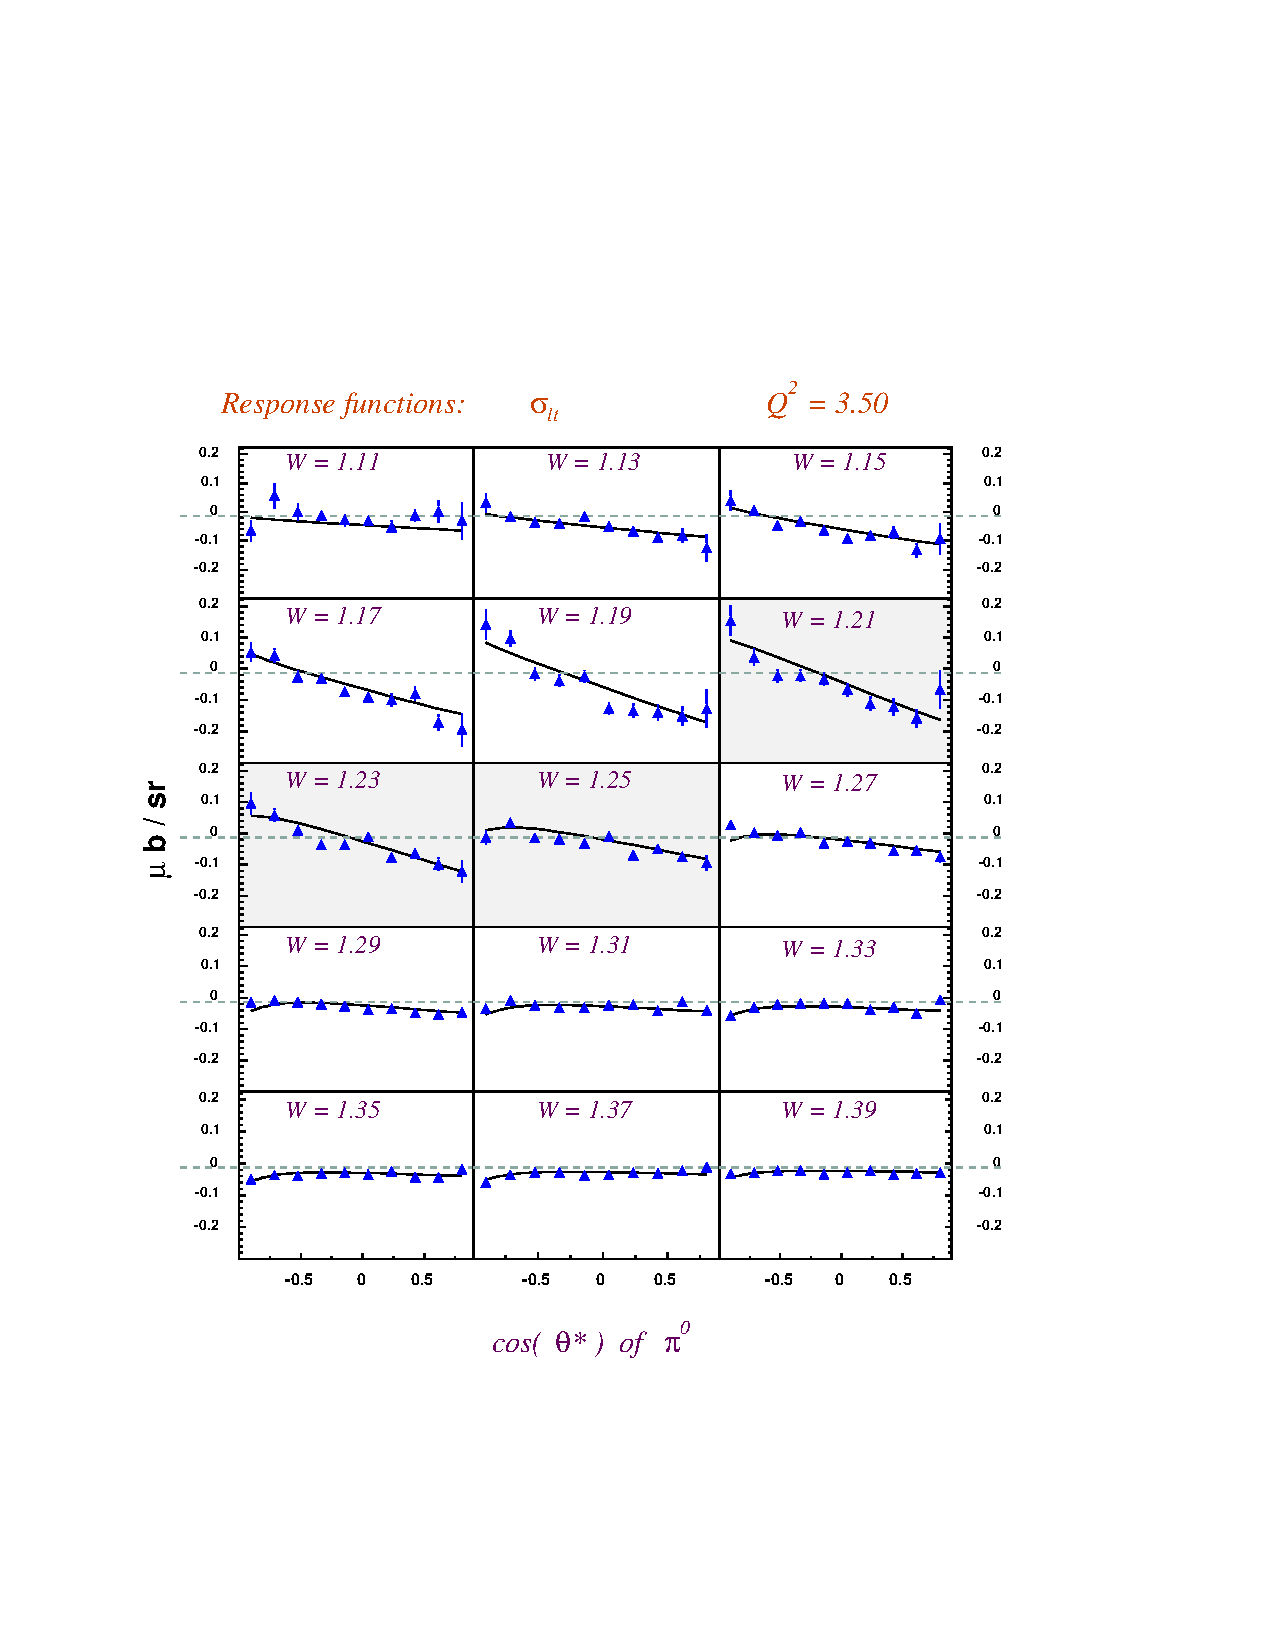
\includegraphics[width = 13cm, bb=-30 140 480 640]{analysis/img/slt_Q23.50_Inn_L1}
  \caption[JANR fit of the cross section: $\sigma_T+\epsilon_L\sigma_L$]
{ JANR fit and  $\sigma_{LT}$. The blue triangles represent the experimental data points. The solid black line
 is the JANR calculated cross section after the JANR fit.}
 \label{fig:lt_Q23.50_Inn_L1}
\end{figure}

\begin{figure}[h]
 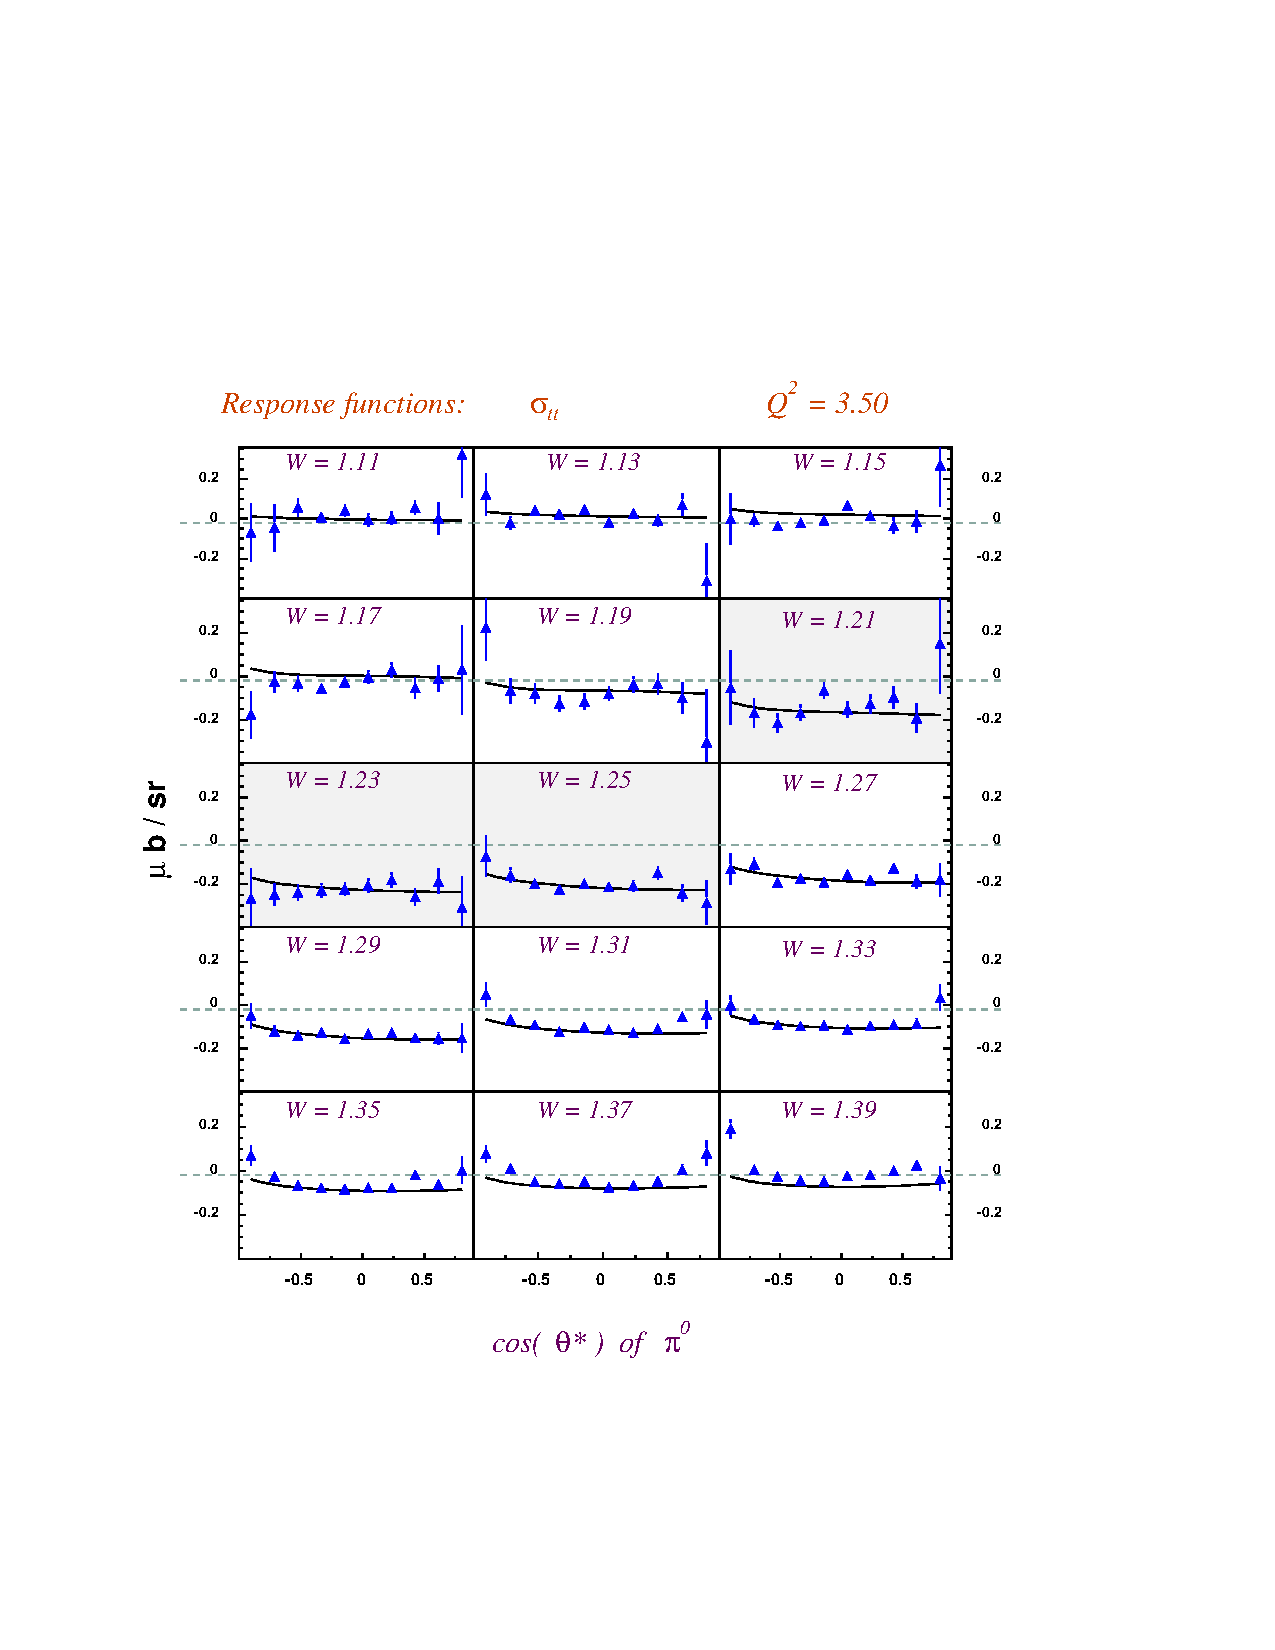
\includegraphics[width = 13cm, bb=-30 140 480 640]{analysis/img/stt_Q23.50_Inn_L1}
  \caption[JANR fit of the cross section: $\sigma_T+\epsilon_L\sigma_L$]
{ JANR fit and  $\sigma_{TT}$. The blue triangles represent the experimental data points. The solid black line
 is the JANR calculated cross section after the JANR fit.}
 \label{fig:tt_Q23.50_Inn_L1}
\end{figure}

\cia  \vspace{-2cm}
\subsection{JANR Results for $R_{EM}$ and $R_{SM}$}
In \F{fig:JANRREM} and \F{fig:JANRRSM} the results for $R_{EM}$ and $R_{SM}$ of the JANR fit is shown.
While $R_{SM}$ is consistent with the multipole truncation result, $R_{EM}$  presents  significantly lower values.
To investigate this discrepancy, the JANR obtained cross section was analyzed using the multipole truncation method.
The result for $R_{EM}$ is shown in \F{fig:JANRREMtrunc}, where one can see that the multipole truncation
introduce a systematic shift on $R_{EM}$, increasing in value with $Q^2$.
The result in \F{fig:JANRREMtrunc} is somewhat consistent with the multipole truncated analysis fit of the experimental 
data shown in \F{fig:RM}.

When comparing the JANR fit of this data with the previous Hall-C data, a significantly smaller value for the 
$M_{1-}$ amplitude is found. See Sec. \ref{sec:other_models}

\begin{figure}[h]
 \begin{center}
 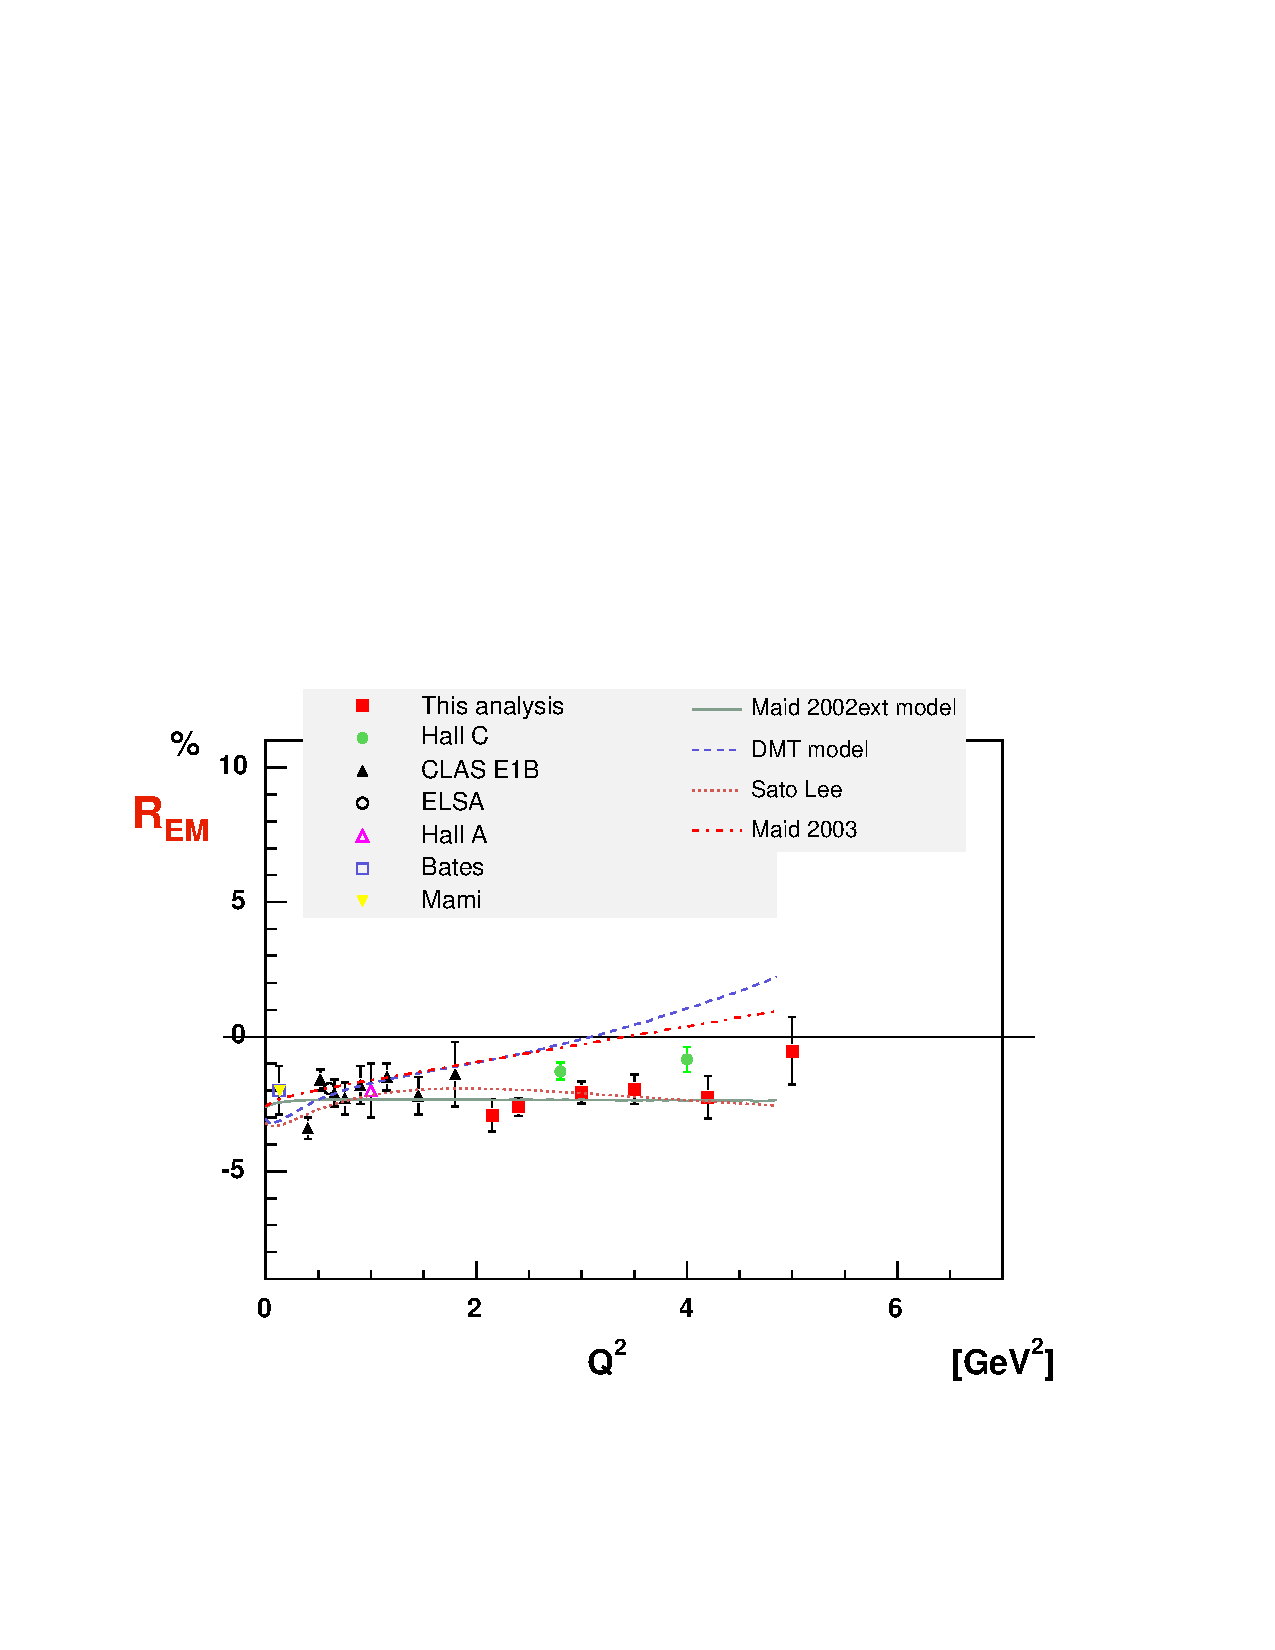
\includegraphics[width = 13cm, bb=30 130 540 500]{analysis/img/JANR_REM} 
  \caption[JANR result for $R_{EM}$ as a function of $Q^2$]
{  Result for $R_{EM}$ as a function of $Q^2$ obtained with JANR.}
 \label{fig:JANRREM}
\end{center}
\end{figure}


\begin{figure}[h]
 \begin{center}
 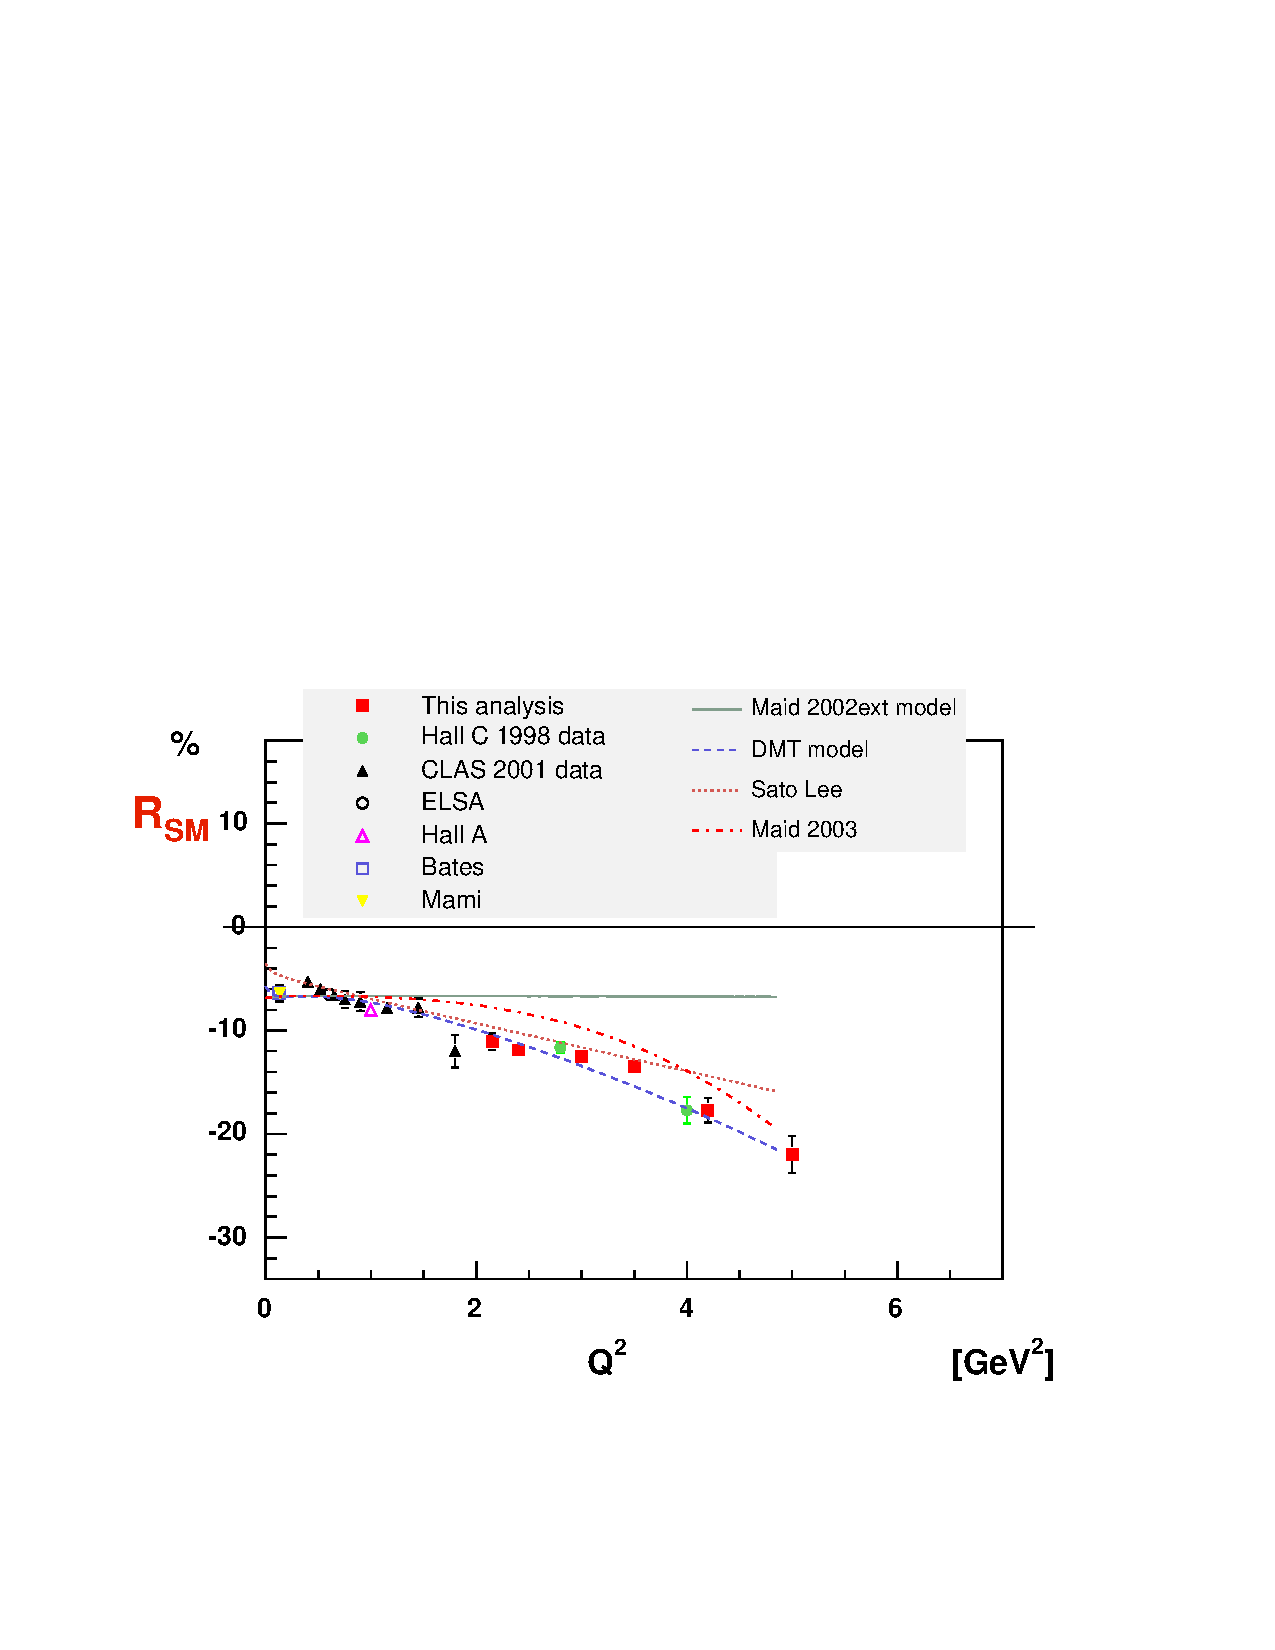
\includegraphics[width = 13cm, bb=30 130 540 500]{analysis/img/JANR_RSM} 
  \caption[JANR result for $R_{SM}$ as a function of $Q^2$]
{  Result for $R_{SM}$ as a function of $Q^2$ obtained with JANR.}
 \label{fig:JANRRSM}
\end{center}
\end{figure}

\begin{figure}[h]
 \begin{center}
 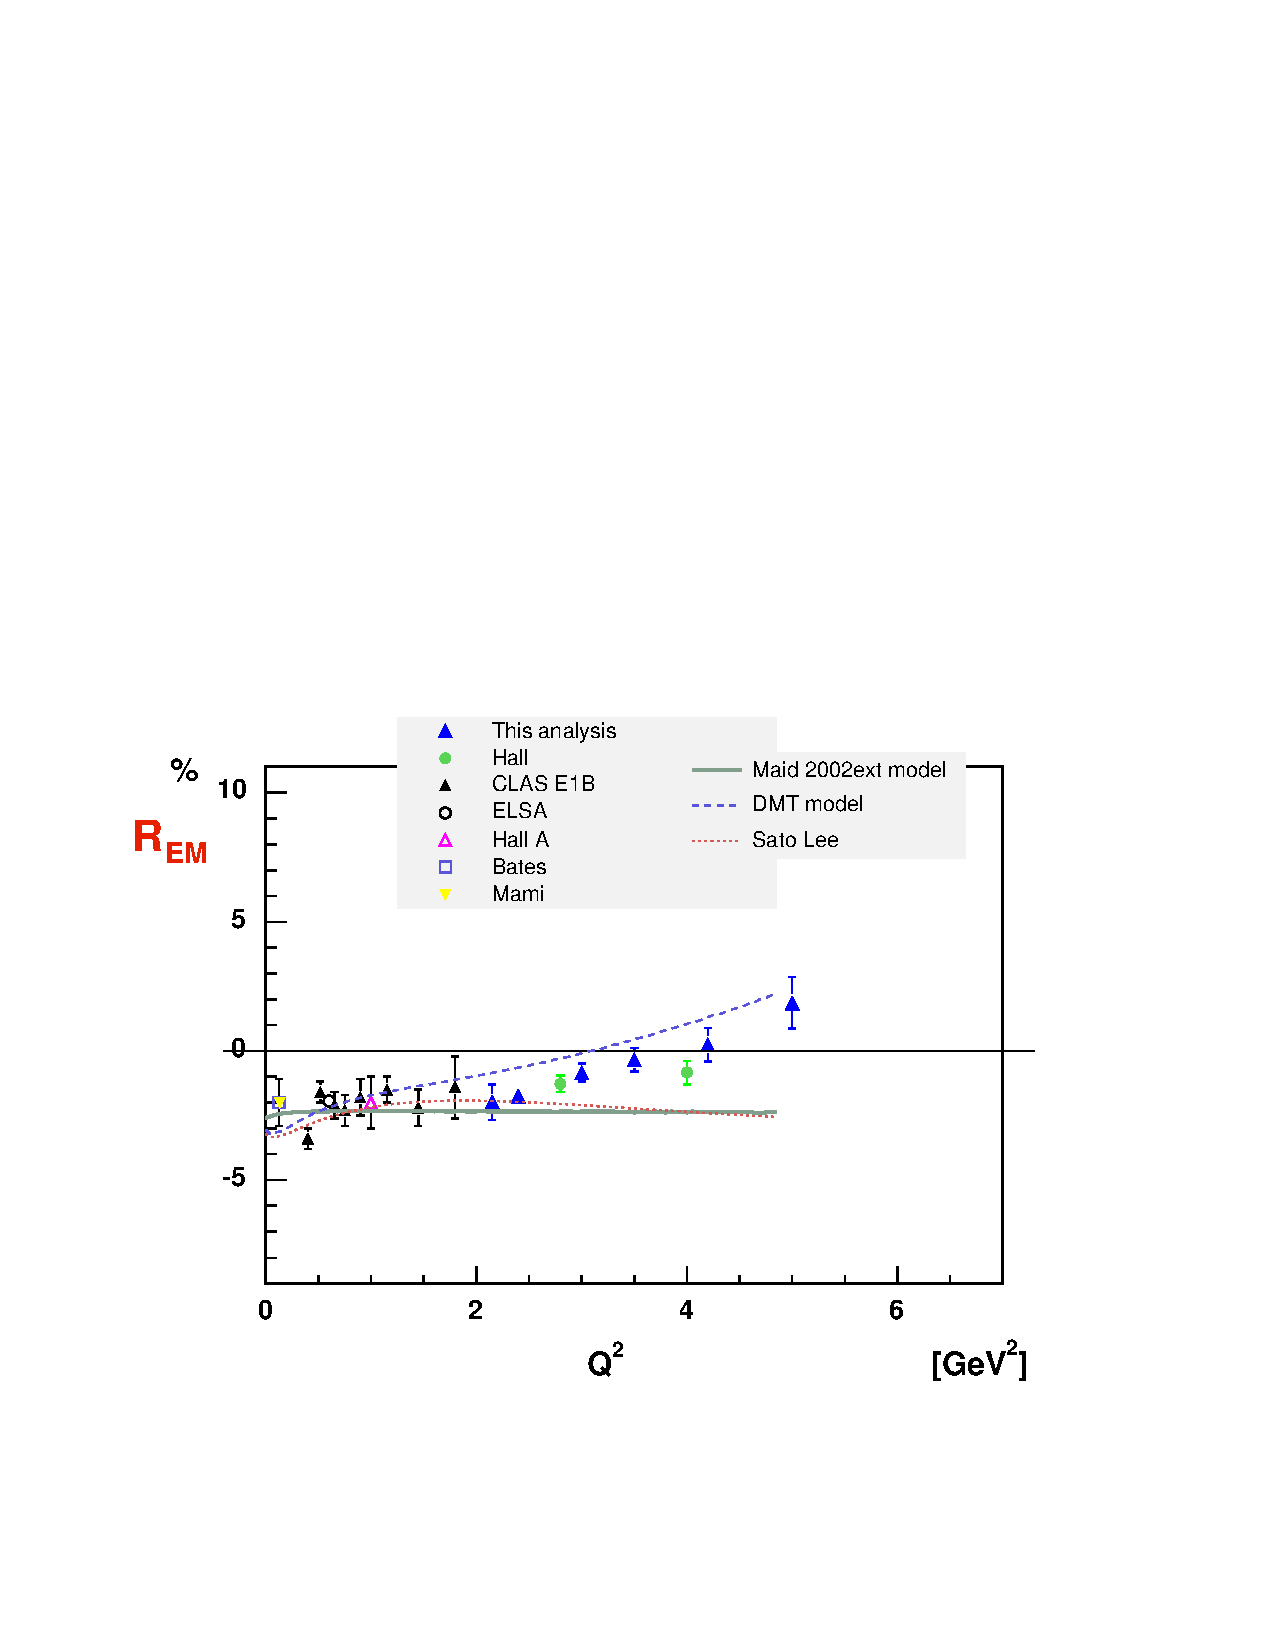
\includegraphics[width = 13cm, bb=30 130 540 500]{analysis/img/JANR_truncated} 
  \caption[JANR truncated result for $R_{EM}$ as a function of $Q^2$]
{  Result for $R_{EM}$ as a function of $Q^2$ obtained applying the multipole truncation method
  to the JANR obtained cross section. Compare this plot with \F{fig:JANRREM} to see how much the 
  result changes with the fit method used. Compare this plot with \F{fig:RM} to see the multipole
  truncation fit to the real data.}
 \label{fig:JANRREMtrunc}
\end{center}
\end{figure}
 

\cia
\section{Different models and the $P_{11}$ signal}\label{sec:other_models}
The data has been compared with the models {\sl maid2000 }, {\sl maid2002ext}, 
{\sl maid2003} \cite{bib:maid2000}\footnote{see also {\tt http://www.kph.uni-mainz.de/MAID } }
{\sl DMT2001} \cite{bib:dmt2001}. When using the maid2003 model, the cross section
has been calculated with or without the $P_{11}$ resonance.
The data has also been compared with the cross section calculated by JANR as a result of the fit
to this data as a check for consistency.
All the cross sections, response functions, coefficient, multipoles distributions can be found
on the web at, respectively:
\begin{verbatim} 
http://www.jlab.org/~ungaro/pi0eprod/cro_plots
http://www.jlab.org/~ungaro/pi0eprod/responses
http://www.jlab.org/~ungaro/pi0eprod/coefficients
http://www.jlab.org/~ungaro/pi0eprod/multipoles
http://www.jlab.org/~ungaro/pi0eprod/results
\end{verbatim}
by clicking the appropriate model check box at the top of the page.

Each model cross section has been fitted as described in Sec. \ref{sec:structure}
and the response functions have been expanded in Legendre polynomial. The coefficents
of the expansion have been compared to the real data.
Here we report the comparison of the $A$ coefficients for the Legendre expansion of
$\sigma_T+\epsilon_L\sigma_L$ at $Q^2=3.5$ $GeV^2$ and $\ell\le 2$.

The JANR fit is a good match to the data, as expected. The coefficient $A_2$ is directly linked
to $R_{EM}$ (see Eq. [\ref{eqno:m1dominance}]). Maid 2002 consistently underestimates $A_2$, 
while DMT matches the data at the $\Delta $ peak, but fails at higher $W$ values.
Good agreement is found for the Maid 2003 model.

When turning on and off the $P_{11}$ resonance in the Maid 2003 model (see \F{fig:A_comp_m03a} and \F{fig:A_comp_m03r})
one can see differences in the $A_0$ and $A_1$ coefficients. Without the Roper resonance Maid 2003 seems to 
better reproduce the data. These behaviour is seen at all $Q^2$. 


\begin{figure}[h]
 \begin{center}
 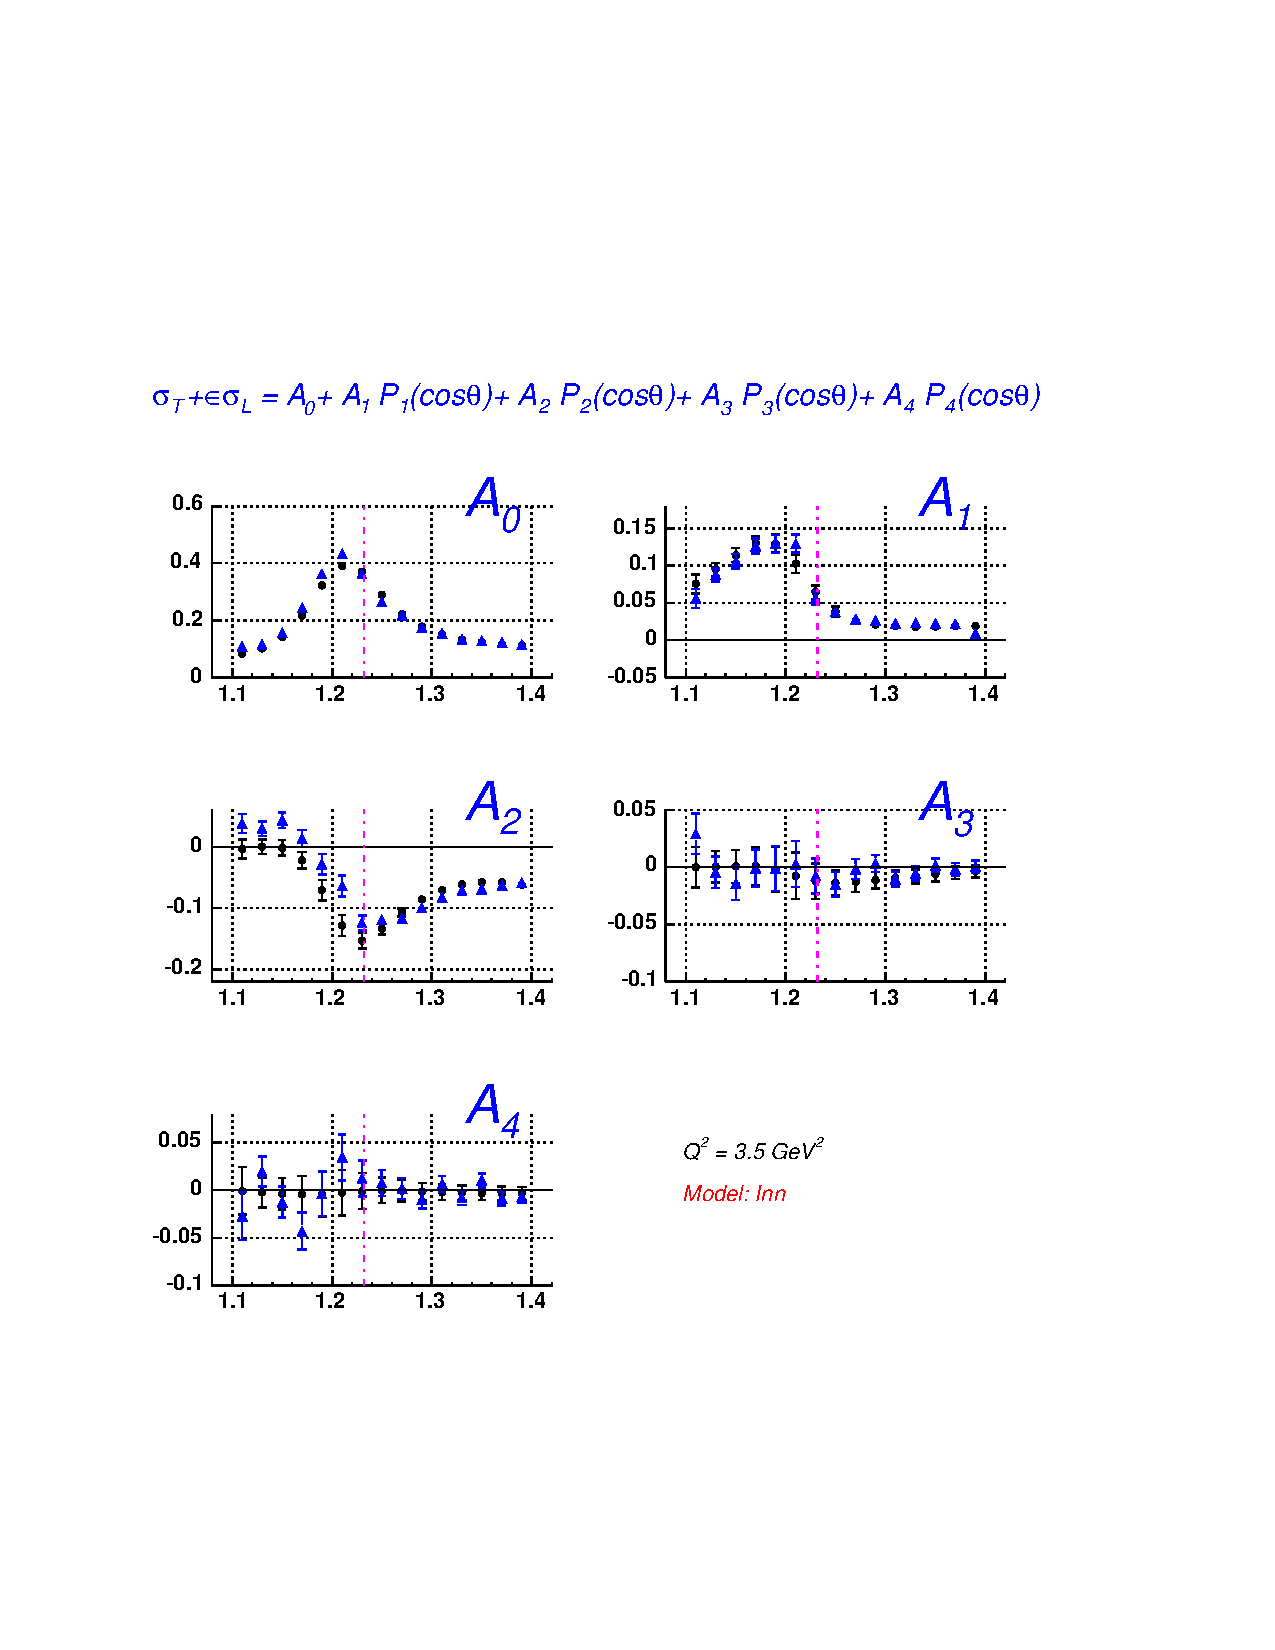
\includegraphics[width = 12cm, bb=30 130 540 700]{analysis/img/A_comp_inna} 
  \caption[Coefficents of the Legendre expansion of $\sigma_T+\epsilon_L\sigma_L$ for the JANR generated cross 
  section  and experimental data ]
{ Coefficents of the Legendre expansion of $\sigma_T+\epsilon_L\sigma_L$ for the JANR generated cross 
  section (black) and experimental data (blue) }
 \label{fig:A_comp_inna}
\end{center}
\end{figure}

\begin{figure}[h]
 \begin{center}
 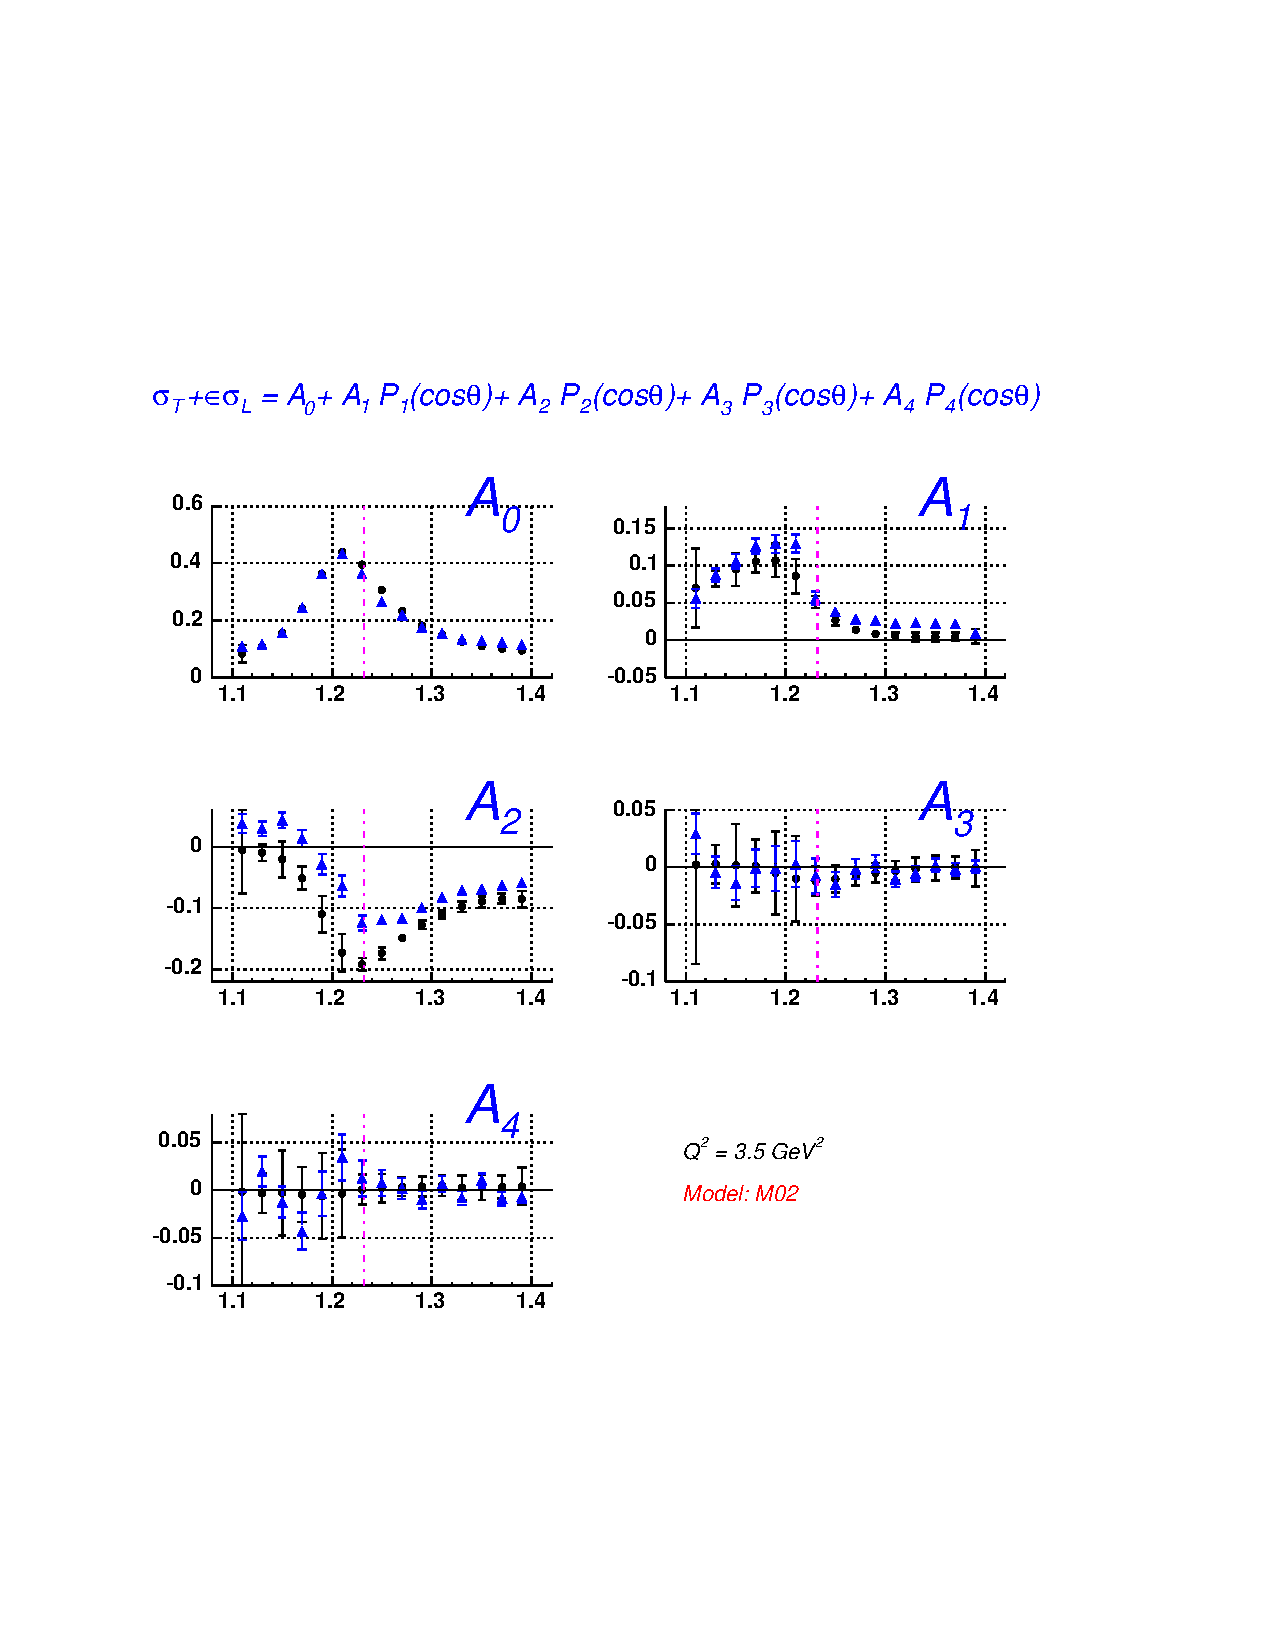
\includegraphics[width = 12cm, bb=30 130 540 700]{analysis/img/A_comp_m02} 
  \caption[Coefficents of the Legendre expansion of $\sigma_T+\epsilon_L\sigma_L$ for the maid 2002 generated cross 
  section  and experimental data ]
{ Coefficents of the Legendre expansion of $\sigma_T+\epsilon_L\sigma_L$ for the maid 2002 generated cross 
  section (black) and experimental data (blue) }
 \label{fig:A_comp_m02}
\end{center}
\end{figure}

\begin{figure}[h]
 \begin{center}
 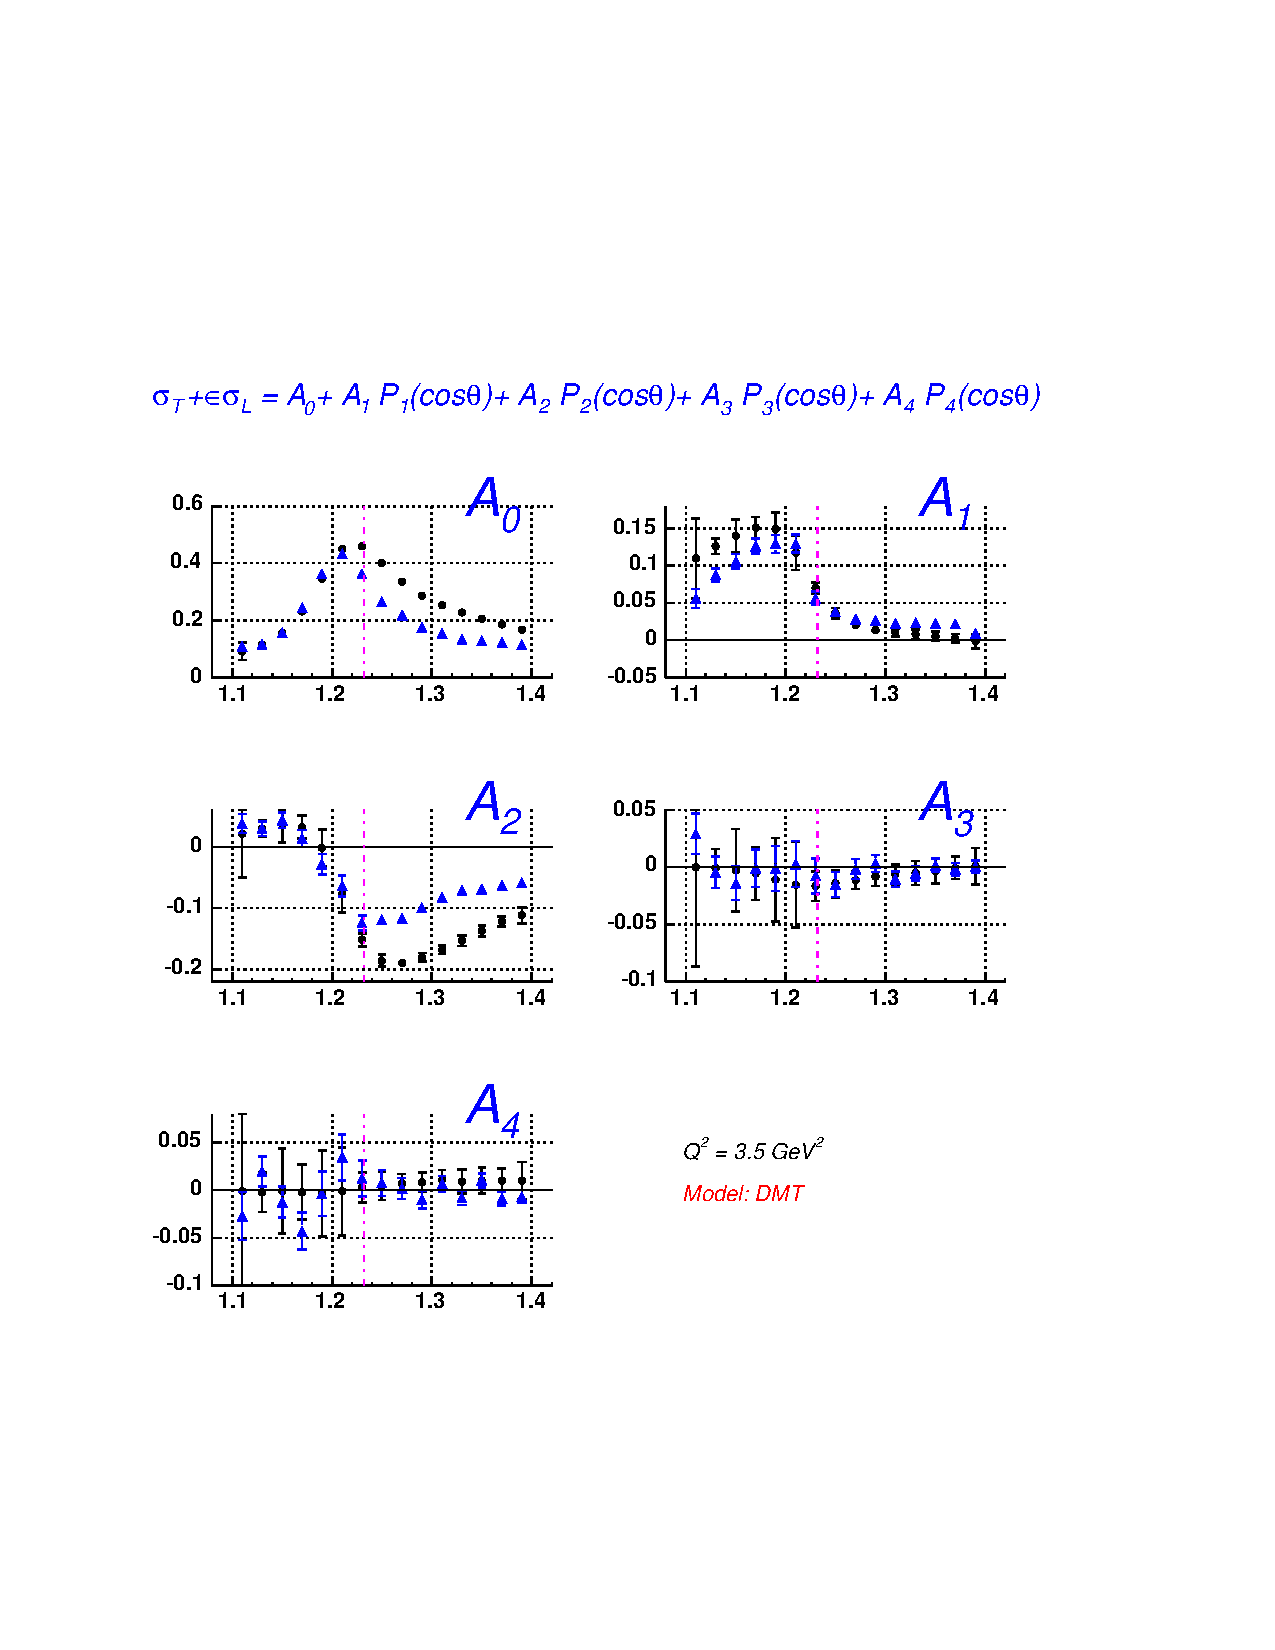
\includegraphics[width = 12cm, bb=30 130 540 700]{analysis/img/A_comp_dmt} 
  \caption[Coefficents of the Legendre expansion of $\sigma_T+\epsilon_L\sigma_L$ for the DMT generated cross 
  section  and experimental data ]
{ Coefficents of the Legendre expansion of $\sigma_T+\epsilon_L\sigma_L$ for the DMT generated cross 
  section (black) and experimental data (blue) }
 \label{fig:A_comp_dmt}
\end{center}
\end{figure}


\begin{figure}[h]
 \begin{center}
 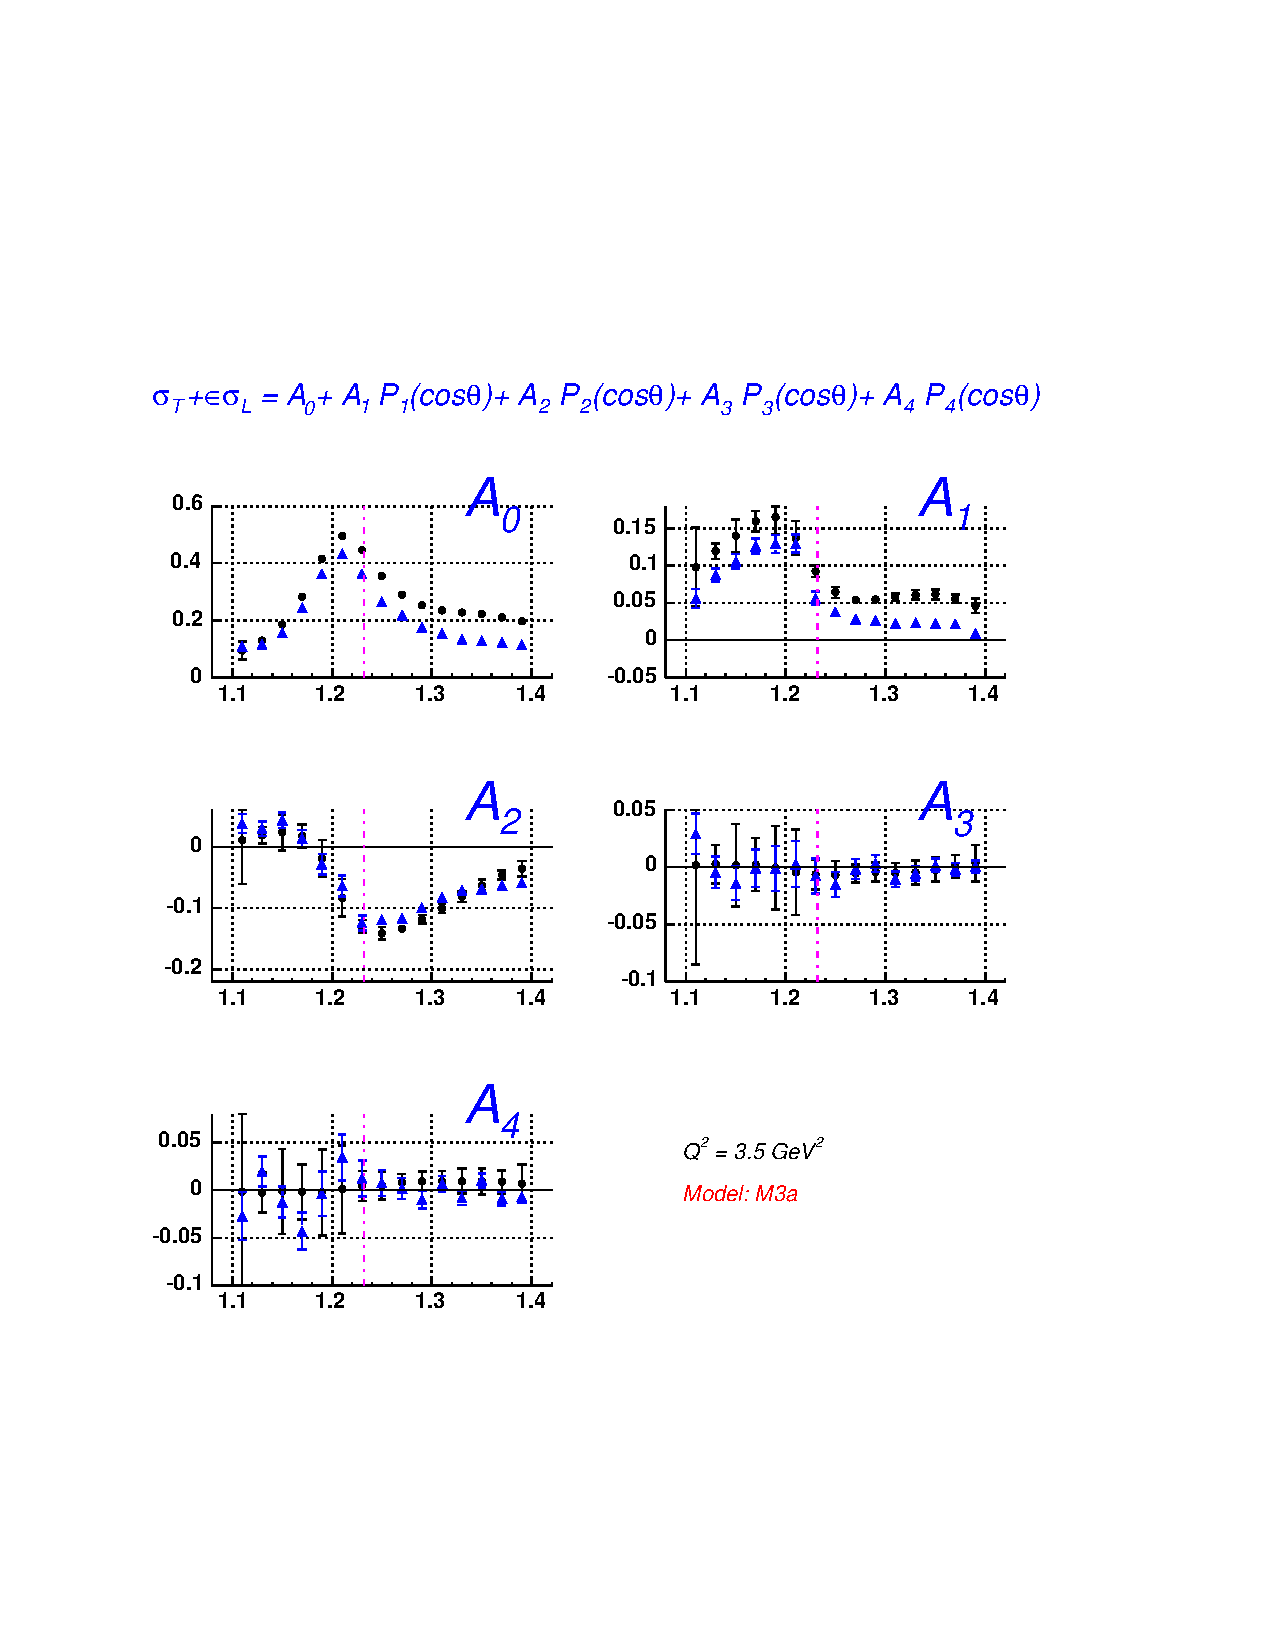
\includegraphics[width = 12cm, bb=30 130 540 700]{analysis/img/A_comp_m03a} 
  \caption[Coefficents of the Legendre expansion of $\sigma_T+\epsilon_L\sigma_L$ for the maid 2003 with Roper {\bf on} 
  generated cross 
  section  and experimental data ]
{ Coefficents of the Legendre expansion of $\sigma_T+\epsilon_L\sigma_L$ for the maid 2003 with Roper {\bf on}  generated cross 
  section (black) and experimental data (blue) }
 \label{fig:A_comp_m03a}
\end{center}
\end{figure}

\begin{figure}[h]
 \begin{center}
 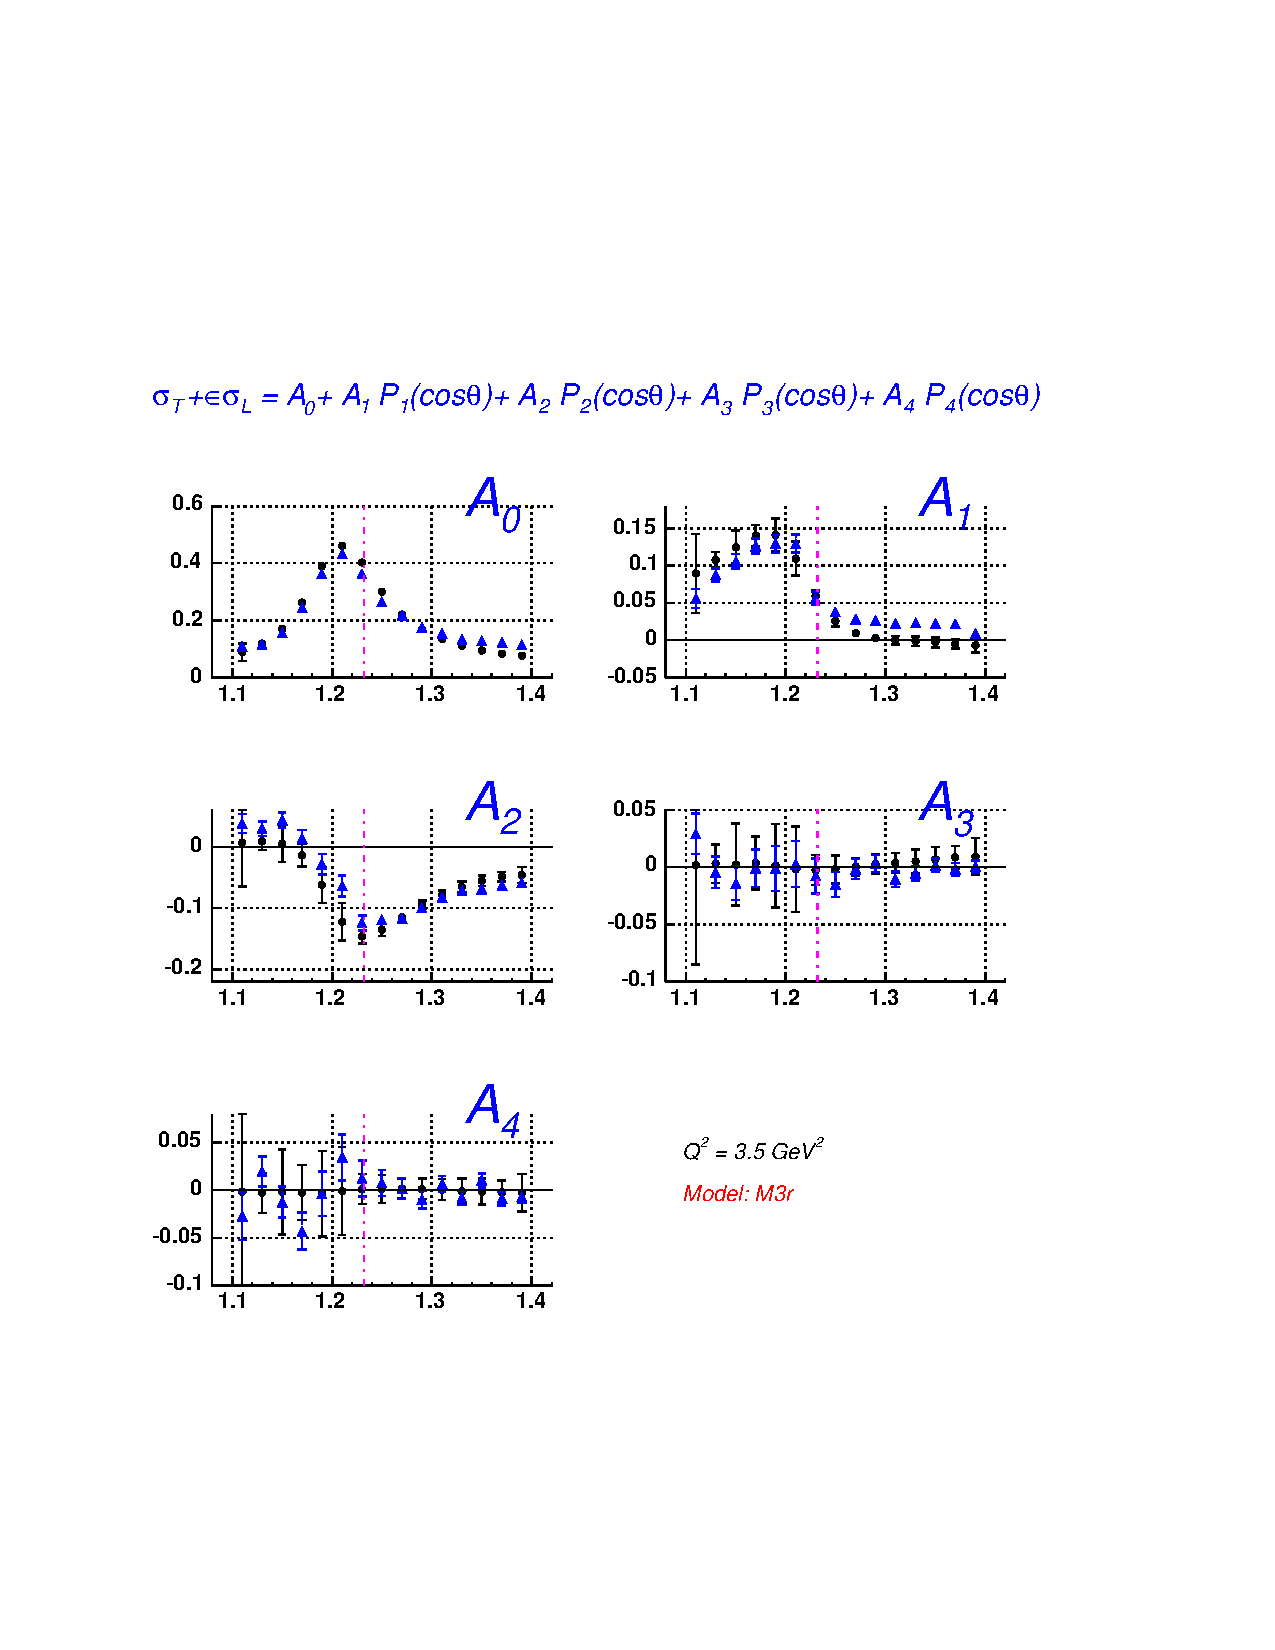
\includegraphics[width = 12cm, bb=30 130 540 700]{analysis/img/A_comp_m03r} 
  \caption[Coefficents of the Legendre expansion of $\sigma_T+\epsilon_L\sigma_L$ for the maid 2003 with Roper {\bf off} 
  generated cross 
  section  and experimental data ]
{ Coefficents of the Legendre expansion of $\sigma_T+\epsilon_L\sigma_L$ for the maid 2003 with Roper {\bf off}  generated cross 
  section (black) and experimental data (blue) }
 \label{fig:A_comp_m03r}
\end{center}
\end{figure}



% \cia
% \section{Discussion}
% The multipoles truncation fit result of $R_{EM}$ suggest a zero crossing between $Q^2$ of $3$ and $4.0$ GeV$^2$.
% This result for $R_{EM}$ would prove that the helicity is not conserved in this range of momentum transferred.
% A recent calculation of the non helicity conserving amplitude in the pQCD framework by Idilbi, 
% 
% The validity of the $M_{1+}$ dominance assumption is questionable, given the fact that the multipoles 
% coming from background and other resonances reach values up to $20-40\% $ of $|M_{1+}|$.
% 
% The result shown in \F{fig:JANRREMtrunc} also suggests that the multipole truncation might not
% be suited to extract the multipoles. 
% 
% The JANR fit  shows a constant negative value of around $-2.5\% $  with the point at $5$ $GeV^2$
% consistent with zero.
% 


